\begin{frame}[t]\frametitle{\problemtitle}
    \begin{block}{Problem}
  	    Given the capacity $1 \leq k \leq 10^9$ of a washing machine with three programmes, and how many items can be washed with which programmes.\\
        What is the minimum number of loads needed to wash all items? 
    \end{block}
    \vspace*{-0.1cm}
    \begin{columns}[b]
        \begin{column}{0.51\textwidth}
    \uncover<2->{
            \begin{block}{Insights}
            \begin{itemize}
                \item<2-> Items with no choice and items with all choices are easy.
                \item<3-> If we assign all items of one set with two choices, an optimal solution for the rest can be determined greedily.  
                % Once we assigned all items of one set with two choices, the optimal solution for the rest can be determined in constant time. 
                \item<5-> There is an optimal solution where there is one set of items with two choices that is assigned to the same programme.      
            \end{itemize}
            \end{block}
    }
        \end{column}
        \hspace{0.3em}
    \begin{column}{0.4\textwidth}
            \begin{figure}
                \only<1>{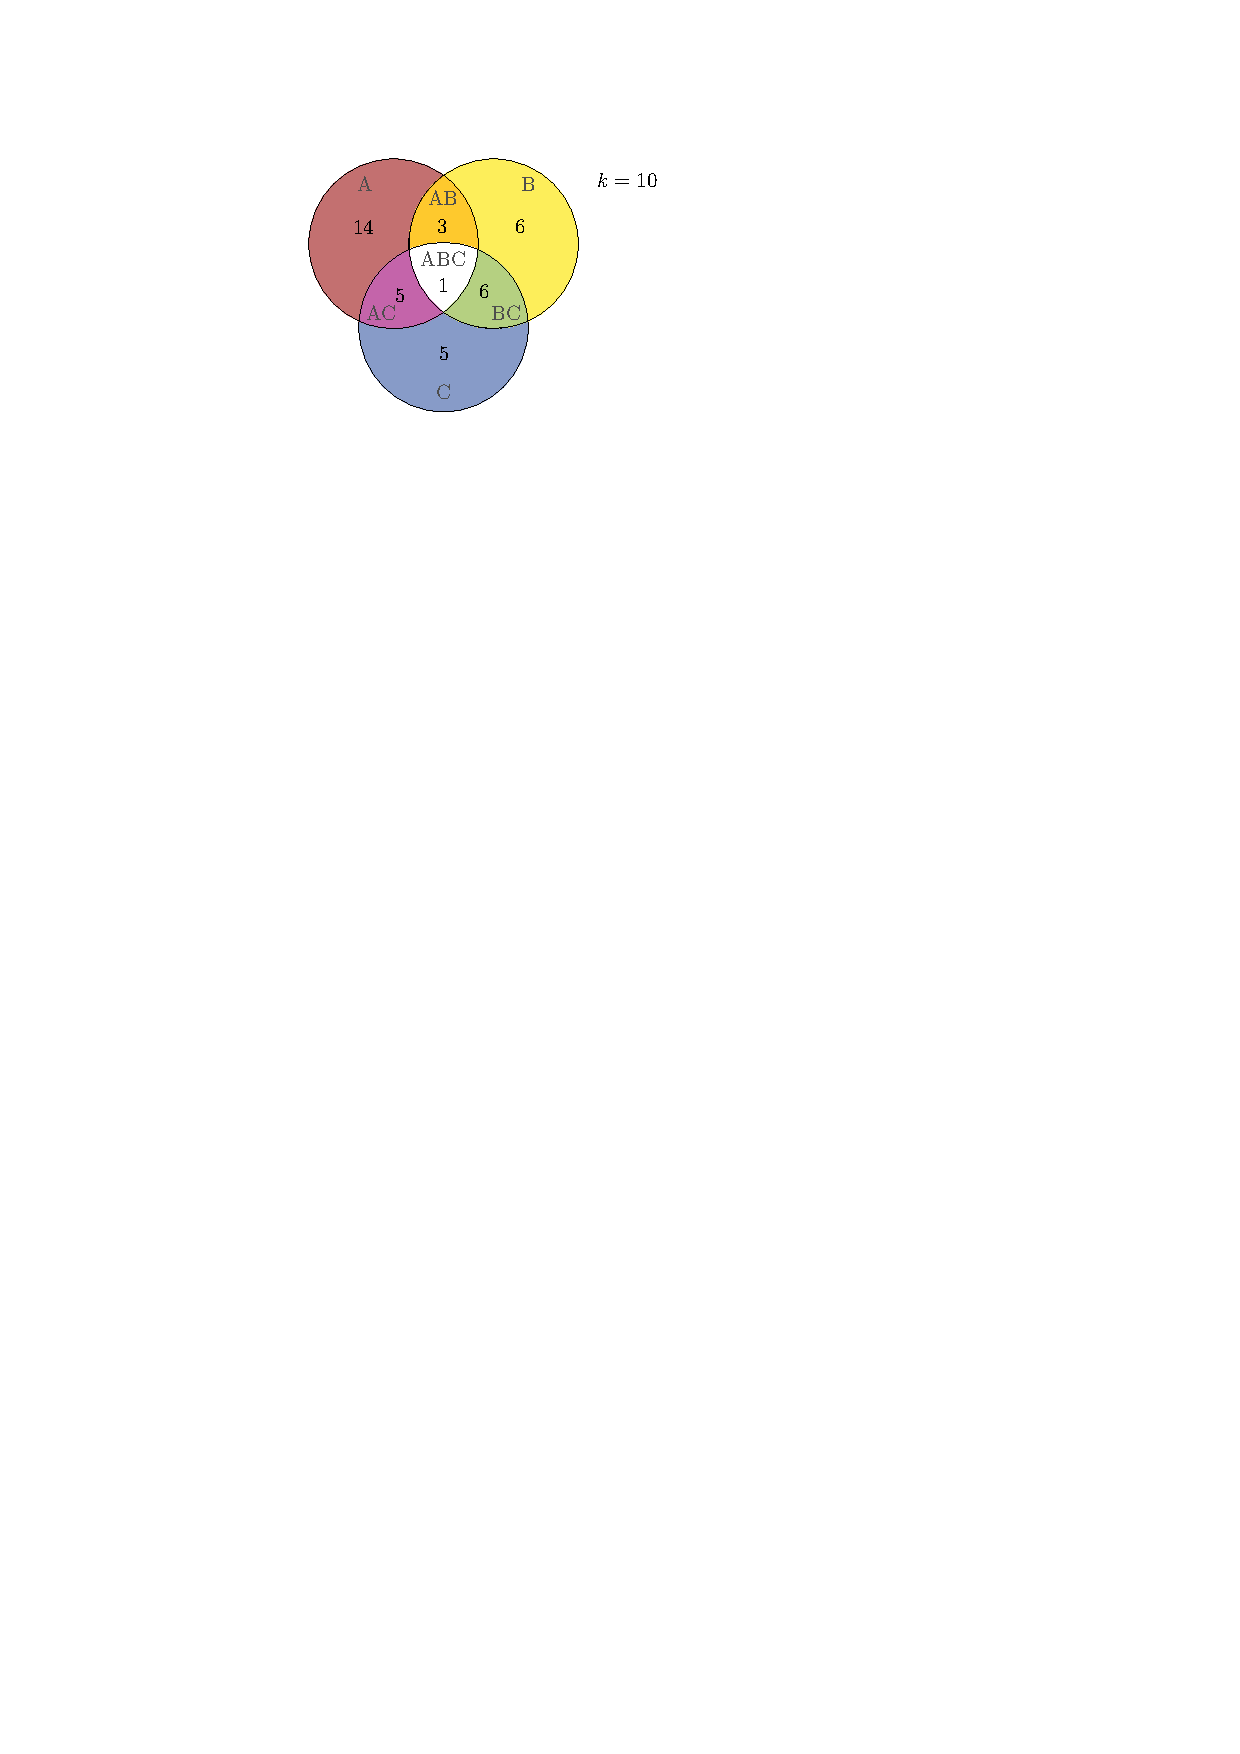
\includegraphics[page=1]{sol}}%
                \only<2>{\includegraphics[page=2]{sol}}%
                \only<3>{\includegraphics[page=3]{sol}}%
                \only<4>{\includegraphics[page=4]{sol}}%
                \only<5>{\includegraphics[page=5]{sol}}%
                \only<6>{\includegraphics[page=6]{sol}}%
            \end{figure}
        \end{column}
    \end{columns}
\end{frame}

\begin{frame}[t]\frametitle{\problemtitle}
    \begin{block}{Problem}
        Given the capacity $1 \leq k \leq 10^9$ of a washing machine with three programmes, and how many items can be washed with which programmes.\\
      What is the minimum number of loads needed to wash all items? 
  \end{block}
  \vspace*{0.3cm}
    \begin{block}{Solution}
        \begin{itemize}
            \item<+-> Process items that can only be washed with one programme first. 
            \item<+-> For each set with two choices: 
            \begin{itemize}
                \item<+-> Try to assign the whole set to one of the two choices.
                \item<+-> Determine the optimal solution for the other sets with two choices. 
                \item<+-> Distribute the items with three choices optimally.
            \end{itemize}
            \item<+-> Take the minimum over all such assignments ($6$ in total). 
        \end{itemize}
        \pause 
        Running time: $\mathcal{O}(1)$ per test case
    \end{block}

    % \solvestats

\end{frame}